% ============================================
% TEMPLATE LAPORAN UTS K3L
% Teknik Fisika - Universitas
% ============================================

\documentclass[12pt,a4paper]{article}

% ========== PACKAGES ==========
\usepackage[utf8]{inputenc}
\usepackage[bahasa]{babel}
\usepackage{geometry}
\usepackage[backend=biber, style=ieee]{biblatex}
\addbibresource{references.bib}
\usepackage{lscape}
\usepackage{pdflscape}
\usepackage{fancyhdr}
\usepackage{graphicx}
\usepackage{setspace}
\usepackage{titlesec}
\usepackage{enumitem}
\usepackage{longtable}
\usepackage{array}
\usepackage{booktabs}
\usepackage{multirow}
\usepackage{xcolor}
\usepackage{hyperref}

% ========== PAGE SETUP ==========
\geometry{
    a4paper,
    left=3cm,
    right=3cm,
    top=3cm,
    bottom=3cm
}

% ========== SPACING ==========
\onehalfspacing

% ========== HEADER & FOOTER ==========
\pagestyle{fancy}
\fancyhf{}
\fancyhead[L]{\small Laporan UTS K3L}
\fancyhead[R]{\small Teknik Fisika}
\fancyfoot[C]{\thepage}
\renewcommand{\headrulewidth}{0.4pt}
\renewcommand{\footrulewidth}{0.4pt}

% =================================================================
% TAMBAHKAN BLOK KODE BARU INI TEPAT DI BAWAH PENGATURAN FANCYHDR
% =================================================================
\fancypagestyle{mylandscape}{
    \fancyhf{} % Hapus semua header dan footer
    \fancyfoot[C]{\thepage} % Atur footer: hanya nomor halaman di tengah
    \renewcommand{\headrulewidth}{0pt} % Pastikan tidak ada garis header
    \renewcommand{\footrulewidth}{0.4pt} % Gambar ulang garis footer
}
% =================================================================

% ========== SECTION FORMATTING ==========
\titleformat{\section}
  {\normalfont\Large\bfseries}{\thesection}{1em}{}
\titleformat{\subsection}
  {\normalfont\large\bfseries}{\thesubsection}{1em}{}
\titleformat{\subsubsection}
  {\normalfont\normalsize\bfseries}{\thesubsubsection}{1em}{}

% ========== HYPERLINK SETUP ==========
\hypersetup{
    colorlinks=true,
    linkcolor=black,
    filecolor=magenta,      
    urlcolor=blue,
    citecolor=blue,
}

% ========== INFORMASI MAHASISWA ==========
% SILAKAN ISI INFORMASI DI BAWAH INI
\newcommand{\mahasiswaNama}{Naufal Haris Nurkhoirulloh}
\newcommand{\mahasiswaNIM}{122140040}
\newcommand{\mahasiswaKelas}{Kelas}
\newcommand{\mahasiswaEmail}{naufal.122140040@student.itera.ac.id}

% ========== DOCUMENT BEGIN ==========
\begin{document}

% Hilangkan header pada halaman cover
\thispagestyle{empty}

% ========== COVER PAGE ==========
% ============================================
% HALAMAN JUDUL (COVER)
% Menggunakan environment 'titlepage' untuk layout yang lebih baik
% ============================================

\begin{titlepage}
    \centering
    \pagestyle{empty} % Memastikan tidak ada header/footer di halaman ini

    \vspace*{1.5cm} % Spasi dari tepi atas

    % --- Judul Utama ---
    {\Large\bfseries MATA KULIAH: K3 DAN LINGKUNGAN KERJA INDUSTRI\par}
    \vspace{1.5em}
    {\Large\bfseries UJIAN TENGAH SEMESTER (UTS)\par}

    \vfill % Memberi spasi fleksibel ke tengah

    % --- Logo ITERA ---
    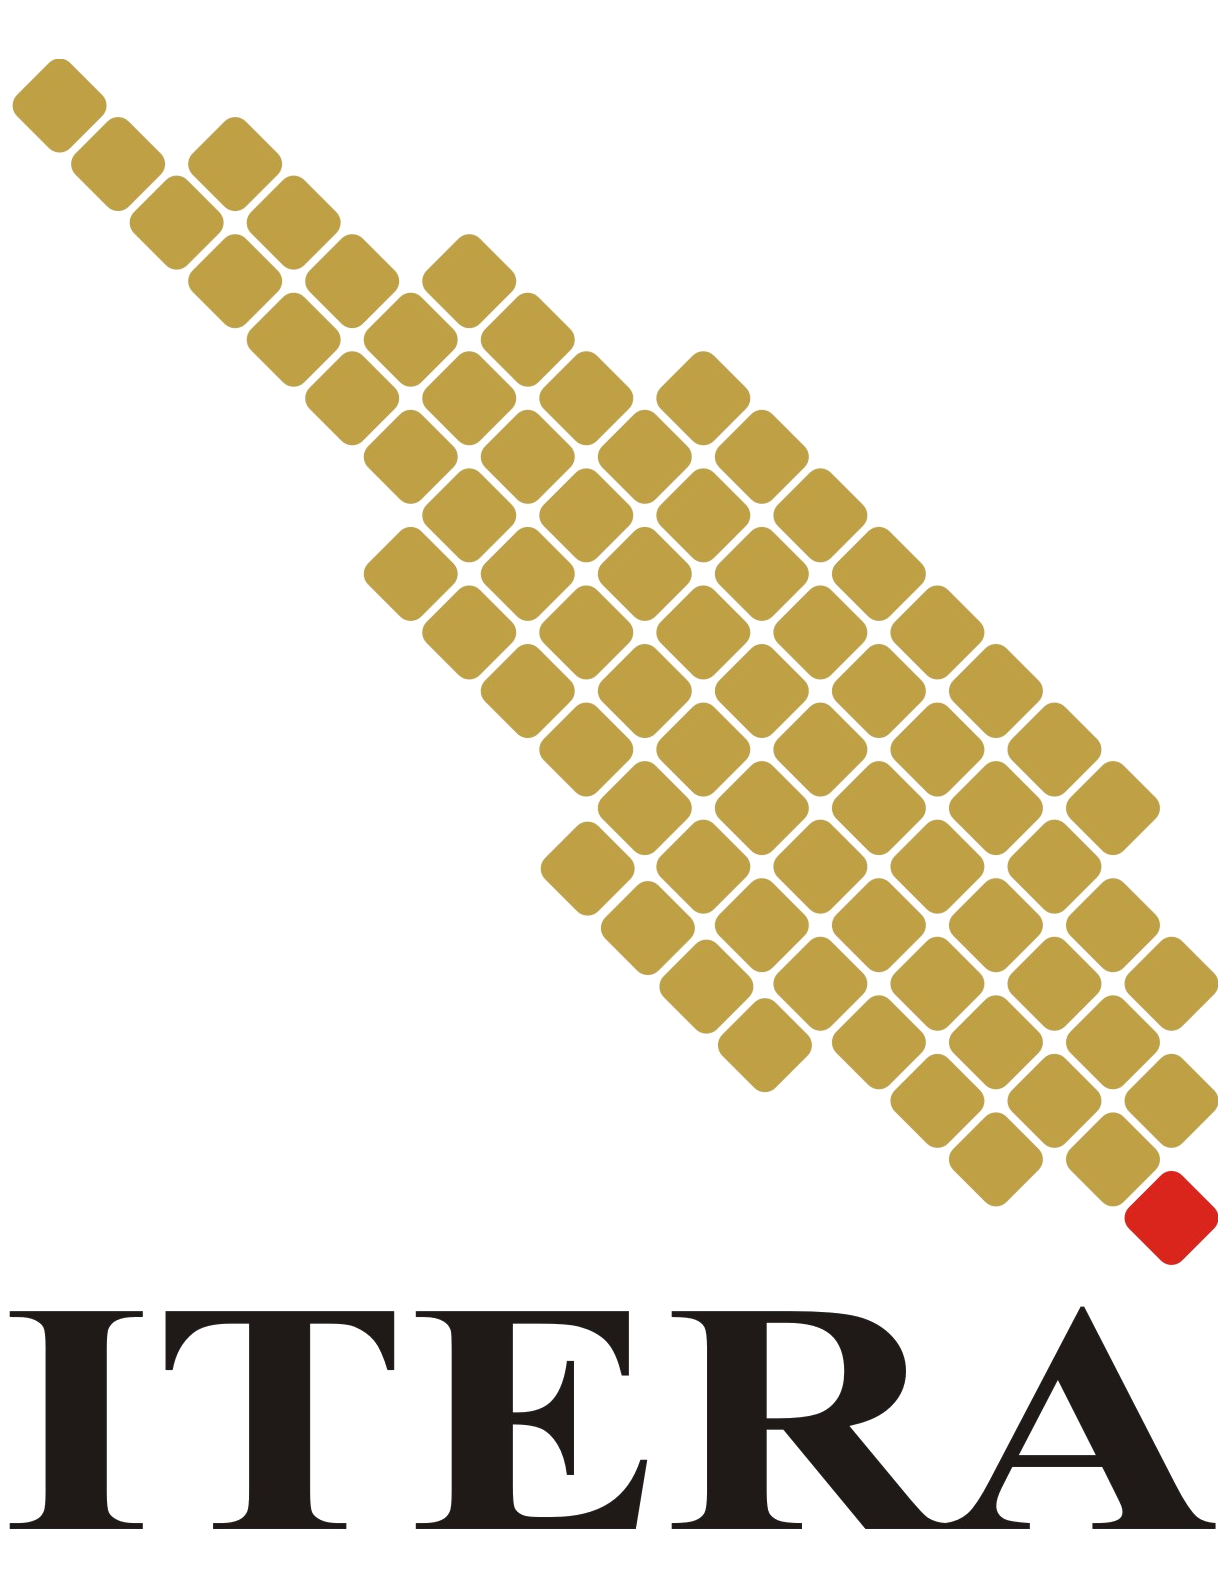
\includegraphics[width=4cm]{figure/Logo_ITERA.png}

    \vfill % Memberi spasi fleksibel ke tengah

    % --- Informasi Mahasiswa dan Dosen ---
    {\large\bfseries Oleh:}\\[2em] % Memberi jarak setelah "Oleh:"
    
    \begin{tabular}{ll}
        \bfseries Nama Mahasiswa & : \mahasiswaNama \\
        \bfseries NIM & : \mahasiswaNIM \\
        \bfseries Dosen Pengampu & : Amrina Mustaqim, S.Si., M.T. \\
    \end{tabular}

    \vfill\vfill % Spasi lebih banyak untuk mendorong bagian bawah

    % --- Informasi Institusi ---
    {\large\bfseries
        PROGRAM STUDI TEKNIK INFORMATIKA \\
        FAKULTAS TEKNOLOGI INDUSTRI\\
        INSTITUT TEKNOLOGI SUMATERA\\
        LAMPUNG SELATAN\\
        \the\year
    }

\end{titlepage}
\newpage

% ========== TABLE OF CONTENTS ==========
\tableofcontents
\newpage

% ========== SOAL 1: KONSEP DAN PERAN K3L ==========
\section{Konsep dan Peran K3L}
\label{sec:konsep-k3l}
% ============================================
% CHAPTER 1: KONSEP DAN PERAN K3L
% Bobot: CPMK5-5 = 25
% ============================================

% JUDUL KASUS - SILAKAN ISI
\subsection*{Judul Kasus: \underline{\hspace{10cm}}}
\addcontentsline{toc}{subsection}{Judul Kasus}

\vspace{0.5cm}

% ========== BAGIAN A: DESKRIPSI SITUASI ==========
\subsection{Deskripsi Situasi}
\label{subsec:deskripsi-situasi}

% Petunjuk:
% - Jelaskan situasi atau kasus K3L yang dipilih secara detail
% - Sertakan data atau pengamatan dari lingkungan sekitar
% - Gunakan bahasa formal dan sistematis
% - Minimal 2-3 paragraf

Jelaskan situasi atau kondisi yang menjadi fokus analisis K3L. Deskripsikan dengan detail meliputi:
\begin{itemize}
    \item Lokasi dan jenis industri/tempat kerja yang diamati
    \item Kondisi aktual yang ditemukan di lapangan
    \item Permasalahan atau potensi bahaya yang teridentifikasi
    \item Data kuantitatif atau kualitatif pendukung
\end{itemize}

\textit{[Tulis deskripsi situasi Anda di sini dengan bahasa formal dan sistematis. Sertakan data observasi dari lingkungan sekitar.]}

\vspace{1cm}

% ========== BAGIAN B: ANALISIS KONSEP K3L ==========
\subsection{Analisis Konsep K3L}
\label{subsec:analisis-konsep}

% Petunjuk:
% - Kaitkan situasi dengan konsep-konsep K3L yang relevan
% - Jelaskan teori/prinsip K3L yang berlaku
% - Analisis bagaimana konsep K3L diterapkan atau diabaikan

Analisis situasi berdasarkan konsep-konsep K3L yang meliputi:

\subsubsection{Keamanan (Security)}
\textit{[Analisis aspek keamanan dalam kasus yang dipilih]}

\subsubsection{Kesehatan Kerja (Occupational Health)}
\textit{[Analisis aspek kesehatan kerja dan dampaknya terhadap pekerja]}

\subsubsection{Keselamatan Kerja (Occupational Safety)}
\textit{[Analisis aspek keselamatan kerja dan potensi kecelakaan]}

\subsubsection{Lingkungan Kerja (Work Environment)}
\textit{[Analisis kondisi lingkungan kerja dan dampak lingkungan]}

\vspace{1cm}

% ========== BAGIAN C: PERAN K3L DI INDUSTRI ==========
\subsection{Peran K3L di Industri}
\label{subsec:peran-k3l}

% Petunjuk:
% - Jelaskan pentingnya K3L dalam konteks industri yang dibahas
% - Diskusikan manfaat implementasi K3L
% - Berikan contoh konkret peran K3L

Uraikan peran dan pentingnya K3L dalam industri/tempat kerja yang dianalisis, meliputi:

\begin{enumerate}[label=\alph*.]
    \item \textbf{Peran Preventif}
    
    \textit{[Jelaskan bagaimana K3L berperan dalam pencegahan kecelakaan dan penyakit akibat kerja]}
    
    \item \textbf{Peran Protektif}
    
    \textit{[Jelaskan bagaimana K3L melindungi pekerja, aset, dan lingkungan]}
    
    \item \textbf{Peran Produktif}
    
    \textit{[Jelaskan hubungan K3L dengan produktivitas dan efisiensi kerja]}
    
    \item \textbf{Peran Legal dan Etis}
    
    \textit{[Jelaskan aspek hukum dan etika dalam implementasi K3L]}
\end{enumerate}

\vspace{1cm}

% ========== BAGIAN D: STRATEGI KOMUNIKASI ==========
\subsection{Strategi Komunikasi}
\label{subsec:strategi-komunikasi}

% Petunjuk:
% - Rancang strategi komunikasi K3L yang efektif
% - Jelaskan metode penyampaian informasi K3L
% - Identifikasi stakeholder dan cara berkomunikasi dengan mereka

Strategi komunikasi K3L yang direkomendasikan untuk kasus ini:

\subsubsection{Identifikasi Stakeholder}
\textit{[Identifikasi pihak-pihak yang terlibat: manajemen, pekerja, kontraktor, dll.]}

\subsubsection{Metode Komunikasi}
\textit{[Jelaskan metode komunikasi yang akan digunakan: briefing, poster, training, dll.]}

Contoh metode komunikasi:
\begin{itemize}
    \item Safety briefing/toolbox meeting
    \item Signage dan rambu-rambu K3L
    \item Sosialisasi dan pelatihan
    \item Media komunikasi internal (bulletin, email, dll.)
    \item Sistem pelaporan bahaya
\end{itemize}

\subsubsection{Media dan Saluran Komunikasi}
\textit{[Tentukan media dan saluran yang paling efektif untuk menyampaikan informasi K3L]}

\subsubsection{Evaluasi Efektivitas Komunikasi}
\textit{[Jelaskan bagaimana mengukur efektivitas strategi komunikasi yang dirancang]}

% ========== CATATAN ==========
% Pastikan semua bagian ditulis dengan:
% - Bahasa formal dan ilmiah
% - Sistematis dan terstruktur
% - Didukung data/referensi yang relevan
% - Minimal rujuk 2-3 sumber literatur
\newpage

% ========== SOAL 2: REGULASI DAN STANDAR K3L ==========
\section{Regulasi dan Standar K3L}
\label{sec:regulasi-k3l}
% ============================================
% CHAPTER 2: REGULASI DAN STANDAR K3L
% Bobot: CPMK5-5 = 25
% ============================================

% JUDUL KASUS - SILAKAN ISI
\subsection*{Judul Kasus: \underline{\hspace{10cm}}}
\addcontentsline{toc}{subsection}{Judul Kasus}

\vspace{0.5cm}

% ========== BAGIAN A: ANALISIS KETERKAITAN REGULASI ==========
\subsection{Analisis Keterkaitan Regulasi}
\label{subsec:analisis-regulasi}

% Petunjuk:
% - Identifikasi regulasi K3L yang relevan dengan kasus
% - Jelaskan bagaimana regulasi tersebut berkaitan dengan situasi
% - Analisis kepatuhan atau ketidakpatuhan terhadap regulasi

Analisis regulasi dan standar K3L yang berkaitan dengan kasus yang dipilih:

\subsubsection{Regulasi Nasional}

\textbf{Undang-Undang yang Relevan:}
\begin{itemize}
    \item UU No. 1 Tahun 1970 tentang Keselamatan Kerja
    \item UU No. 13 Tahun 2003 tentang Ketenagakerjaan
    \item UU No. 32 Tahun 2009 tentang Perlindungan dan Pengelolaan Lingkungan Hidup
    \item \textit{[Tambahkan UU lain yang relevan]}
\end{itemize}

\textit{[Jelaskan pasal-pasal spesifik yang terkait dengan kasus Anda]}

\vspace{0.5cm}

\textbf{Peraturan Pemerintah dan Peraturan Menteri:}
\begin{itemize}
    \item PP No. 50 Tahun 2012 tentang Penerapan SMK3
    \item Permenaker No. 5 Tahun 2018 tentang K3 Lingkungan Kerja
    \item Permenaker No. 8 Tahun 2020 tentang Alat Pelindung Diri
    \item \textit{[Tambahkan peraturan lain yang relevan]}
\end{itemize}

\textit{[Analisis bagaimana peraturan-peraturan ini berkaitan dengan kasus]}

\vspace{0.5cm}

\subsubsection{Standar Internasional}

\textbf{Standar ISO dan OHSAS:}
\begin{itemize}
    \item ISO 45001:2018 - Sistem Manajemen Kesehatan dan Keselamatan Kerja
    \item ISO 14001:2015 - Sistem Manajemen Lingkungan
    \item \textit{[Tambahkan standar lain yang relevan]}
\end{itemize}

\textit{[Jelaskan penerapan atau ketidaksesuaian dengan standar internasional]}

\vspace{0.5cm}

\subsubsection{Standar Industri Spesifik}

\textit{[Identifikasi standar khusus untuk industri yang dibahas, misalnya: standar kelistrikan, standar konstruksi, standar laboratorium, dll.]}

\vspace{0.5cm}

\subsubsection{Analisis Kepatuhan}

Berdasarkan observasi dan data yang dikumpulkan, analisis kepatuhan terhadap regulasi:

\begin{table}[h]
\centering
\begin{tabular}{|p{5cm}|p{3cm}|p{6cm}|}
\hline
\textbf{Aspek Regulasi} & \textbf{Status Kepatuhan} & \textbf{Keterangan} \\
\hline
\textit{[Contoh: Penyediaan APD]} & \textit{[Patuh/Tidak]} & \textit{[Penjelasan detail]} \\
\hline
 & & \\
\hline
 & & \\
\hline
 & & \\
\hline
\end{tabular}
\caption{Analisis Kepatuhan Regulasi K3L}
\label{tab:kepatuhan-regulasi}
\end{table}

\textit{[Tambahkan penjelasan narasi tentang temuan kepatuhan]}

\vspace{1cm}

% ========== BAGIAN B: LANGKAH PERBAIKAN SISTEM ==========
\subsection{Langkah Perbaikan Sistem}
\label{subsec:perbaikan-sistem}

% Petunjuk:
% - Rancang langkah-langkah konkret untuk memperbaiki sistem K3L
% - Prioritaskan perbaikan berdasarkan tingkat urgensi dan risiko
% - Sertakan timeline dan resources yang dibutuhkan

Berdasarkan analisis regulasi dan kepatuhan, berikut langkah perbaikan sistem K3L:

\subsubsection{Perbaikan Jangka Pendek (0-3 bulan)}

\begin{enumerate}
    \item \textbf{Perbaikan Segera (Emergency)}
    
    \textit{[Identifikasi masalah kritis yang memerlukan tindakan segera]}
    
    \begin{itemize}
        \item Masalah: \textit{[Deskripsikan]}
        \item Tindakan: \textit{[Deskripsikan]}
        \item Penanggung jawab: \textit{[Sebutkan]}
        \item Target waktu: \textit{[Tentukan]}
    \end{itemize}
    
    \item \textbf{Perbaikan Prioritas Tinggi}
    
    \textit{[Masalah yang perlu diperbaiki dalam waktu dekat]}
\end{enumerate}

\vspace{0.5cm}

\subsubsection{Perbaikan Jangka Menengah (3-6 bulan)}

\textit{[Uraikan program perbaikan yang memerlukan perencanaan lebih matang]}

\begin{itemize}
    \item Pengembangan sistem manajemen K3L
    \item Upgrading fasilitas dan peralatan
    \item Implementasi program kesehatan kerja
    \item \textit{[Tambahkan poin lainnya]}
\end{itemize}

\vspace{0.5cm}

\subsubsection{Perbaikan Jangka Panjang (6-12 bulan)}

\textit{[Uraikan program strategis dan berkelanjutan]}

\begin{itemize}
    \item Sertifikasi ISO 45001
    \item Budaya keselamatan (safety culture)
    \item Sistem monitoring dan evaluasi berkelanjutan
    \item \textit{[Tambahkan poin lainnya]}
\end{itemize}

\vspace{0.5cm}

\subsubsection{Rencana Implementasi}

\begin{table}[h]
\centering
\small
\begin{tabular}{|c|p{4cm}|p{3cm}|c|p{2.5cm}|}
\hline
\textbf{No} & \textbf{Langkah Perbaikan} & \textbf{Penanggung Jawab} & \textbf{Timeline} & \textbf{Resources} \\
\hline
1 & \textit{[Langkah 1]} & \textit{[PJ]} & \textit{[Waktu]} & \textit{[Sumber daya]} \\
\hline
2 & & & & \\
\hline
3 & & & & \\
\hline
4 & & & & \\
\hline
5 & & & & \\
\hline
\end{tabular}
\caption{Rencana Implementasi Perbaikan Sistem K3L}
\label{tab:rencana-implementasi}
\end{table}

\vspace{1cm}

% ========== BAGIAN C: PERAN KOMUNIKASI & PELATIHAN ==========
\subsection{Peran Komunikasi dan Pelatihan}
\label{subsec:komunikasi-pelatihan}

% Petunjuk:
% - Jelaskan pentingnya komunikasi dalam implementasi regulasi
% - Rancang program pelatihan K3L
% - Identifikasi metode komunikasi yang efektif

\subsubsection{Peran Komunikasi dalam Implementasi Regulasi}

\textit{[Jelaskan bagaimana komunikasi efektif mendukung penerapan regulasi K3L]}

Aspek-aspek komunikasi yang perlu diperhatikan:
\begin{itemize}
    \item Sosialisasi peraturan dan kebijakan K3L
    \item Penyampaian perubahan regulasi terbaru
    \item Sistem pelaporan dan feedback
    \item Komunikasi antar level organisasi
\end{itemize}

\vspace{0.5cm}

\subsubsection{Program Pelatihan K3L}

\textbf{A. Analisis Kebutuhan Pelatihan}

\textit{[Identifikasi gap kompetensi dan kebutuhan pelatihan]}

\vspace{0.3cm}

\textbf{B. Rancangan Program Pelatihan}

\begin{table}[h]
\centering
\small
\begin{tabular}{|c|p{4cm}|p{3cm}|p{2cm}|p{2cm}|}
\hline
\textbf{No} & \textbf{Jenis Pelatihan} & \textbf{Target Peserta} & \textbf{Durasi} & \textbf{Frekuensi} \\
\hline
1 & Induksi K3L & Karyawan baru & 4 jam & Sekali \\
\hline
2 & K3L Umum & Semua karyawan & 8 jam & Tahunan \\
\hline
3 & \textit{[Pelatihan spesifik]} & \textit{[Target]} & \textit{[Durasi]} & \textit{[Frekuensi]} \\
\hline
4 & & & & \\
\hline
\end{tabular}
\caption{Program Pelatihan K3L}
\label{tab:program-pelatihan}
\end{table}

\vspace{0.3cm}

\textbf{C. Metode Pelatihan}

\begin{itemize}
    \item Classroom training
    \item On-the-job training
    \item E-learning
    \item Simulasi dan drill
    \item \textit{[Tambahkan metode lainnya]}
\end{itemize}

\vspace{0.5cm}

\subsubsection{Evaluasi Efektivitas Komunikasi dan Pelatihan}

\textit{[Jelaskan metode evaluasi untuk mengukur efektivitas program komunikasi dan pelatihan]}

\begin{itemize}
    \item Pre-test dan post-test
    \item Observasi perilaku kerja
    \item Survey kepuasan peserta
    \item Monitoring indikator K3L (frequency rate, severity rate, dll.)
    \item \textit{[Tambahkan metode evaluasi lainnya]}
\end{itemize}

% ========== CATATAN ==========
% Pastikan semua bagian ditulis dengan:
% - Merujuk pada regulasi yang spesifik dan terbaru
% - Data dan fakta yang dapat diverifikasi
% - Rencana yang realistis dan dapat diimplementasikan
% - Bahasa formal dan sistematis
\newpage

% ========== SOAL 3: IDENTIFIKASI BAHAYA DAN ANALISIS RISIKO ==========
\section{Identifikasi Bahaya dan Analisis Risiko}
\label{sec:identifikasi-bahaya}
% ============================================
% CHAPTER 3: IDENTIFIKASI BAHAYA DAN ANALISIS RISIKO
% Bobot: CPMK5-6 = 25
% ============================================

% ========== BAGIAN A: IDENTIFIKASI JENIS BAHAYA ==========
\subsection{Identifikasi Jenis Bahaya}
\label{subsec:identifikasi-bahaya}

% Petunjuk:
% - Identifikasi berbagai jenis bahaya di tempat kerja
% - Klasifikasikan bahaya berdasarkan kategorinya
% - Berikan deskripsi detail untuk setiap bahaya

Berdasarkan observasi dan inspeksi di lokasi kerja, berikut identifikasi jenis-jenis bahaya yang ditemukan:

\subsubsection{Bahaya Fisik (Physical Hazards)}

\textit{[Identifikasi bahaya fisik yang ada di tempat kerja]}

Contoh bahaya fisik yang perlu diidentifikasi:
\begin{itemize}
    \item Kebisingan (noise)
    \item Getaran (vibration)
    \item Pencahayaan tidak memadai
    \item Suhu ekstrem (panas atau dingin)
    \item Radiasi (ionisasi atau non-ionisasi)
    \item Tekanan tidak normal
    \item \textit{[Tambahkan bahaya fisik lain yang ditemukan]}
\end{itemize}

\vspace{0.5cm}

\subsubsection{Bahaya Kimia (Chemical Hazards)}

\textit{[Identifikasi bahaya kimia yang ada di tempat kerja]}

Contoh bahaya kimia:
\begin{itemize}
    \item Bahan kimia beracun
    \item Gas berbahaya
    \item Debu dan partikel
    \item Uap dan aerosol
    \item Bahan mudah terbakar
    \item Bahan korosif
    \item \textit{[Tambahkan bahaya kimia lain yang ditemukan]}
\end{itemize}

\vspace{0.5cm}

\subsubsection{Bahaya Biologi (Biological Hazards)}

\textit{[Identifikasi bahaya biologi yang ada di tempat kerja]}

Contoh bahaya biologi:
\begin{itemize}
    \item Bakteri dan virus
    \item Jamur dan spora
    \item Parasit
    \item Hewan berbahaya
    \item Limbah medis/biologis
    \item \textit{[Tambahkan bahaya biologi lain yang ditemukan]}
\end{itemize}

\vspace{0.5cm}

\subsubsection{Bahaya Ergonomi (Ergonomic Hazards)}

\textit{[Identifikasi bahaya ergonomi yang ada di tempat kerja]}

Contoh bahaya ergonomi:
\begin{itemize}
    \item Postur kerja tidak ergonomis
    \item Gerakan berulang (repetitive motion)
    \item Pengangkatan manual beban berat
    \item Workstation tidak sesuai
    \item Durasi kerja berlebihan
    \item \textit{[Tambahkan bahaya ergonomi lain yang ditemukan]}
\end{itemize}

\vspace{0.5cm}

\subsubsection{Bahaya Psikososial (Psychosocial Hazards)}

\textit{[Identifikasi bahaya psikososial yang ada di tempat kerja]}

Contoh bahaya psikososial:
\begin{itemize}
    \item Stres kerja
    \item Beban kerja berlebihan
    \item Kekerasan di tempat kerja
    \item Shift kerja tidak teratur
    \item Kurangnya dukungan sosial
    \item \textit{[Tambahkan bahaya psikososial lain yang ditemukan]}
\end{itemize}

\vspace{0.5cm}

\subsubsection{Bahaya Mekanik (Mechanical Hazards)}

\textit{[Identifikasi bahaya mekanik yang ada di tempat kerja]}

Contoh bahaya mekanik:
\begin{itemize}
    \item Mesin bergerak tanpa pelindung
    \item Alat potong dan tajam
    \item Bagian berputar (rotating parts)
    \item Peralatan bertekanan
    \item Kendaraan dan alat berat
    \item \textit{[Tambahkan bahaya mekanik lain yang ditemukan]}
\end{itemize}

\vspace{0.5cm}

\subsubsection{Bahaya Listrik (Electrical Hazards)}

\textit{[Identifikasi bahaya listrik yang ada di tempat kerja]}

Contoh bahaya listrik:
\begin{itemize}
    \item Kontak langsung dengan arus listrik
    \item Instalasi listrik tidak standar
    \item Kabel rusak atau tidak terproteksi
    \item Grounding tidak memadai
    \item Overload listrik
    \item \textit{[Tambahkan bahaya listrik lain yang ditemukan]}
\end{itemize}

\vspace{1cm}

% ========== BAGIAN B: ANALISIS RISIKO ==========
\subsection{Analisis Risiko}
\label{subsec:analisis-risiko}

% Petunjuk:
% - Gunakan metode risk assessment (misalnya: Risk Matrix 5x5)
% - Tentukan nilai kemungkinan (likelihood) dan keparahan (severity)
% - Hitung tingkat risiko dan prioritaskan pengendalian

\subsubsection{Metode Penilaian Risiko}

Analisis risiko dilakukan menggunakan metode \textit{Risk Matrix 5x5} dengan kriteria sebagai berikut:

\textbf{Kriteria Kemungkinan (Likelihood):}
\begin{itemize}
    \item Nilai 1 (Sangat Jarang): Hampir tidak pernah terjadi (< 1 kali/10 tahun)
    \item Nilai 2 (Jarang): Pernah terjadi di industri sejenis (1 kali/5-10 tahun)
    \item Nilai 3 (Kadang-kadang): Dapat terjadi (1 kali/1-5 tahun)
    \item Nilai 4 (Sering): Sering terjadi (beberapa kali/tahun)
    \item Nilai 5 (Sangat Sering): Sangat sering terjadi (beberapa kali/bulan)
\end{itemize}

\textbf{Kriteria Keparahan (Severity):}
\begin{itemize}
    \item Nilai 1 (Dapat Diabaikan): Tidak ada cidera, kerugian minimal
    \item Nilai 2 (Minor): Cidera ringan, P3K, kerugian kecil
    \item Nilai 3 (Sedang): Cidera sedang, perlu perawatan medis, kerugian sedang
    \item Nilai 4 (Major): Cidera berat, cacat permanen, kerugian besar
    \item Nilai 5 (Catastrophic): Kematian, cacat total, kerugian sangat besar
\end{itemize}

\textbf{Tingkat Risiko:}
\begin{itemize}
    \item Risiko Rendah (1-4): Dapat diterima dengan monitoring
    \item Risiko Sedang (5-9): Perlu tindakan pengendalian
    \item Risiko Tinggi (10-15): Perlu tindakan segera
    \item Risiko Sangat Tinggi (16-25): Hentikan aktivitas sampai risiko terkendali
\end{itemize}

\vspace{0.5cm}

\subsubsection{Tabel Analisis Risiko}

\clearpage 
\begin{landscape}
    \thispagestyle{empty} % <<< INI PERINTAHNYA: Menghilangkan semua header & footer
    
    \begin{longtable}{|c|p{3cm}|p{3.5cm}|p{3.5cm}|c|c|c|p{4cm}|}
        \caption{Analisis Risiko K3L} \label{tab:analisis-risiko} \\
        \hline
        \textbf{No} & \textbf{Jenis Bahaya} & \textbf{Sumber Bahaya} & \textbf{Potensi Akibat} & \textbf{Nilai Kemungkinan (L)} & \textbf{Nilai Keparahan (S)} & \textbf{Tingkat Risiko (LxS)} & \textbf{Rekomendasi Pengendalian} \\
        \hline
        \endfirsthead
        
        \multicolumn{8}{c}%
        {\tablename\ \thetable\ -- \textit{Lanjutan dari halaman sebelumnya}} \\
        \hline
        \textbf{No} & \textbf{Jenis Bahaya} & \textbf{Sumber Bahaya} & \textbf{Potensi Akibat} & \textbf{Nilai Kemungkinan (L)} & \textbf{Nilai Keparahan (S)} & \textbf{Tingkat Risiko (LxS)} & \textbf{Rekomendasi Pengendalian} \\
        \hline
        \endhead

        \hline
        \multicolumn{8}{r}{\textit{Bersambung ke halaman berikutnya}} \\
        \endfoot

        \hline
        \endlastfoot

        1 & \textit{[Contoh: Kebisingan]} & \textit{[Mesin produksi]} & \textit{[Gangguan pendengaran]} & \textit{4} & \textit{3} & \textit{12 (Tinggi)} & \textit{[APD earplug/earmuff, enclosure mesin]} \\
        \hline
        2 & & & & & & & \\ \hline
        3 & & & & & & & \\ \hline
        4 & & & & & & & \\ \hline
        5 & & & & & & & \\ \hline
        6 & & & & & & & \\ \hline
        7 & & & & & & & \\ \hline
        8 & & & & & & & \\ \hline
        9 & & & & & & & \\ \hline
        10 & & & & & & & \\ \hline
    \end{longtable}
\end{landscape}
\clearpage

\vspace{0.5cm}

\subsubsection{Risk Matrix}

\begin{table}[h]
\centering
\begin{tabular}{|c|c|c|c|c|c|}
\hline
\multirow{2}{*}{\textbf{Keparahan (S)}} & \multicolumn{5}{c|}{\textbf{Kemungkinan (L)}} \\
\cline{2-6}
 & \textbf{1} & \textbf{2} & \textbf{3} & \textbf{4} & \textbf{5} \\
\hline
\textbf{5} & 5 & 10 & 15 & 20 & 25 \\
\hline
\textbf{4} & 4 & 8 & 12 & 16 & 20 \\
\hline
\textbf{3} & 3 & 6 & 9 & 12 & 15 \\
\hline
\textbf{2} & 2 & 4 & 6 & 8 & 10 \\
\hline
\textbf{1} & 1 & 2 & 3 & 4 & 5 \\
\hline
\end{tabular}
\caption{Risk Matrix 5x5}
\label{tab:risk-matrix}
\end{table}

\textbf{Keterangan Warna:}
\begin{itemize}
    \item Hijau (1-4): Risiko Rendah
    \item Kuning (5-9): Risiko Sedang
    \item Oranye (10-15): Risiko Tinggi
    \item Merah (16-25): Risiko Sangat Tinggi
\end{itemize}

\vspace{1cm}

% ========== BAGIAN C: ALAT BANTU IDENTIFIKASI BAHAYA ==========
\subsection{Alat Bantu Identifikasi Bahaya}
\label{subsec:alat-bantu}

% Petunjuk:
% - Jelaskan alat/metode yang digunakan untuk identifikasi bahaya
% - Diskusikan kelebihan dan kekurangan masing-masing alat
% - Berikan contoh penerapan

\subsubsection{Metode Identifikasi Bahaya}

Dalam melakukan identifikasi bahaya dan analisis risiko, digunakan beberapa metode dan alat bantu:

\textbf{1. Job Safety Analysis (JSA)}

\textit{[Jelaskan penggunaan JSA dalam mengidentifikasi bahaya pada setiap langkah pekerjaan]}

Kelebihan:
\begin{itemize}
    \item Analisis detail per langkah kerja
    \item Mudah dipahami pekerja
    \item Dapat digunakan sebagai bahan pelatihan
\end{itemize}

\textbf{2. Hazard and Operability Study (HAZOP)}

\textit{[Jelaskan jika menggunakan metode HAZOP, terutama untuk proses industri]}

\textbf{3. What-If Analysis}

\textit{[Jelaskan penggunaan analisis What-If untuk brainstorming bahaya potensial]}

\textbf{4. Checklist Inspeksi K3L}

\textit{[Jelaskan penggunaan checklist untuk inspeksi rutin]}

Contoh checklist yang digunakan:
\begin{itemize}
    \item Checklist area kerja
    \item Checklist peralatan dan mesin
    \item Checklist APD
    \item Checklist housekeeping
\end{itemize}

\textbf{5. Safety Walk-Through}

\textit{[Jelaskan metode observasi langsung di lapangan]}

\textbf{6. Failure Mode and Effect Analysis (FMEA)}

\textit{[Jelaskan jika menggunakan FMEA untuk analisis kegagalan sistem]}

\vspace{0.5cm}

\subsubsection{Tools dan Teknologi Pendukung}

\textit{[Jelaskan alat bantu teknologi yang digunakan]}

\begin{itemize}
    \item Software HIRA (Hazard Identification and Risk Assessment)
    \item Alat ukur lingkungan kerja (sound level meter, lux meter, dll.)
    \item Aplikasi mobile untuk pelaporan bahaya
    \item Database bahaya dan risiko
    \item \textit{[Tambahkan tools lain yang digunakan]}
\end{itemize}

\vspace{0.5cm}

\subsubsection{Dokumentasi dan Pelaporan}

\textit{[Jelaskan sistem dokumentasi identifikasi bahaya]}

\begin{itemize}
    \item Format laporan identifikasi bahaya
    \item Sistem penyimpanan dan updating data
    \item Komunikasi hasil identifikasi kepada stakeholder
    \item Review dan update berkala
\end{itemize}

% ========== CATATAN ==========
% Pastikan:
% - Tabel analisis risiko diisi dengan data observasi nyata
% - Perhitungan tingkat risiko akurat
% - Rekomendasi pengendalian mengikuti hirarki kontrol
% - Semua bagian didukung dengan data dan referensi
\newpage

% ========== SOAL 4: PENERAPAN SOP & SIKAP AKADEMIK ==========
\section{Penerapan SOP dan Sikap Akademik}
\label{sec:penerapan-sop}
% ============================================
% CHAPTER 4: PENERAPAN SOP & SIKAP AKADEMIK
% Bobot: CPMK5-6 = 25
% ============================================

% ========== BAGIAN A: RANCANGAN SINGKAT SOP ==========
\subsection{Rancangan Singkat SOP}
\label{subsec:rancangan-sop}

% Petunjuk:
% - Buat SOP yang spesifik untuk kasus yang dipilih
% - Gunakan bahasa yang jelas, sistematis, dan operasional
% - Sertakan langkah-langkah detail dengan penanggung jawab

\subsubsection{Informasi Umum SOP}

\begin{table}[h]
\centering
\begin{tabular}{|p{4cm}|p{9cm}|}
\hline
\textbf{Judul SOP} & \textit{[Isi judul SOP sesuai kasus, contoh: "SOP Pengoperasian Mesin Bubut"]} \\
\hline
\textbf{Nomor Dokumen} & \textit{[Contoh: SOP/K3L/001/2025]} \\
\hline
\textbf{Tanggal Berlaku} & \textit{[Tanggal efektif]} \\
\hline
\textbf{Revisi} & \textit{[Nomor revisi, contoh: Rev. 00]} \\
\hline
\textbf{Disusun Oleh} & \textit{[Nama penyusun]} \\
\hline
\textbf{Disetujui Oleh} & \textit{[Nama yang menyetujui]} \\
\hline
\textbf{Unit Kerja} & \textit{[Nama unit/departemen]} \\
\hline
\end{tabular}
\caption{Informasi Dokumen SOP}
\label{tab:info-sop}
\end{table}

\vspace{0.5cm}

\subsubsection{Tujuan SOP}

\textit{[Jelaskan tujuan dari SOP ini, misalnya:]}
\begin{itemize}
    \item Memastikan keselamatan pekerja dalam melakukan aktivitas
    \item Meminimalkan risiko kecelakaan kerja
    \item Menjamin konsistensi prosedur kerja
    \item Memenuhi persyaratan regulasi K3L
\end{itemize}

\vspace{0.5cm}

\subsubsection{Ruang Lingkup}

\textit{[Jelaskan cakupan penerapan SOP, misalnya:]}
\begin{itemize}
    \item Area kerja yang tercakup
    \item Personel yang terlibat
    \item Aktivitas yang diatur
    \item Batasan-batasan penerapan
\end{itemize}

\vspace{0.5cm}

\subsubsection{Definisi dan Istilah}

\textit{[Jelaskan istilah-istilah khusus yang digunakan dalam SOP]}

\begin{itemize}
    \item \textbf{APD}: Alat Pelindung Diri
    \item \textbf{JSA}: Job Safety Analysis
    \item \textbf{LOTO}: Lock Out Tag Out
    \item \textit{[Tambahkan definisi lain yang relevan]}
\end{itemize}

\vspace{0.5cm}

\subsubsection{Referensi}

\textit{[Sebutkan dokumen atau regulasi yang menjadi acuan]}

\begin{itemize}
    \item UU No. 1 Tahun 1970 tentang Keselamatan Kerja
    \item ISO 45001:2018
    \item \textit{[Tambahkan referensi lain]}
\end{itemize}

\vspace{1cm}

\subsubsection{Prosedur Kerja}

\clearpage
\begin{landscape}
    \thispagestyle{empty} % <<< INI PERINTAHNYA: Menghilangkan semua header & footer
    
    \begin{longtable}{|c|p{5cm}|p{3cm}|p{4cm}|p{4cm}|}
        \caption{Langkah-Langkah SOP K3L} \label{tab:langkah-sop} \\
        \hline
        \textbf{Langkah} & \textbf{Deskripsi Tindakan} & \textbf{Penanggung Jawab} & \textbf{Alat yang Digunakan} & \textbf{Catatan K3L} \\
        \hline
        \endfirsthead
        
        \multicolumn{5}{c}%
        {\tablename\ \thetable\ -- \textit{Lanjutan dari halaman sebelumnya}} \\
        \hline
        \textbf{Langkah} & \textbf{Deskripsi Tindakan} & \textbf{Penanggung Jawab} & \textbf{Alat yang Digunakan} & \textbf{Catatan K3L} \\
        \hline
        \endhead

        \hline
        \multicolumn{5}{r}{\textit{Bersambung ke halaman berikutnya}} \\
        \endfoot

        \hline
        \endlastfoot

        % ... (semua baris tabel Anda) ...
        \hline
    \end{longtable}
    
\end{landscape}
\clearpage  

\vspace{0.5cm}

\subsubsection{APD yang Diperlukan}

\begin{table}[h]
\centering
\begin{tabular}{|c|p{4cm}|p{6cm}|p{3cm}|}
\hline
\textbf{No} & \textbf{Jenis APD} & \textbf{Fungsi} & \textbf{Standar} \\
\hline
1 & Safety Helmet & Melindungi kepala dari benturan & SNI, ANSI \\
\hline
2 & Safety Shoes & Melindungi kaki dari tertimpa benda & SNI \\
\hline
3 & Safety Glasses & Melindungi mata dari percikan & ANSI Z87.1 \\
\hline
4 & \textit{[Tambahkan APD lain]} & & \\
\hline
\end{tabular}
\caption{Daftar APD yang Diperlukan}
\label{tab:apd-sop}
\end{table}

\vspace{0.5cm}

\subsubsection{Kondisi Darurat}

\textit{[Jelaskan prosedur jika terjadi kondisi darurat]}

\begin{enumerate}
    \item \textbf{Stop Work}: Hentikan pekerjaan segera
    \item \textbf{Secure Area}: Amankan area kerja
    \item \textbf{Report}: Laporkan ke supervisor/HSE
    \item \textbf{Emergency Response}: Lakukan tindakan darurat sesuai jenis insiden
    \item \textbf{Investigation}: Lakukan investigasi kecelakaan
\end{enumerate}

\vspace{0.5cm}

\subsubsection{Review dan Update SOP}

\textit{[Jelaskan mekanisme review dan update SOP]}

\begin{itemize}
    \item Review berkala: minimal 1 tahun sekali
    \item Review insidental: jika terjadi perubahan proses atau insiden
    \item Approval: SOP harus disetujui oleh manajemen
    \item Sosialisasi: SOP baru harus disosialisasikan ke semua pihak terkait
\end{itemize}

\vspace{1cm}

% ========== BAGIAN B: SIKAP AKADEMIK DAN KOMUNIKATIF ==========
\subsection{Sikap Akademik dan Komunikatif}
\label{subsec:sikap-akademik}

% Petunjuk:
% - Refleksikan proses pembelajaran dalam mengerjakan UTS
% - Tunjukkan sikap aktif, analitis, inovatif, dan bertanggung jawab
% - Evaluasi kemampuan komunikasi dalam menyusun laporan

\subsubsection{Refleksi Proses Pembelajaran}

\textit{[Tuliskan refleksi pribadi tentang proses pembelajaran K3L]}

\textbf{A. Pemahaman Konsep K3L}

\textit{[Jelaskan bagaimana pemahaman Anda tentang K3L berkembang selama perkuliahan dan dalam mengerjakan UTS ini]}

Aspek-aspek yang dipelajari:
\begin{itemize}
    \item Konsep dasar K3L dan penerapannya
    \item Regulasi dan standar yang berlaku
    \item Metode identifikasi bahaya dan analisis risiko
    \item Penyusunan SOP yang efektif
    \item \textit{[Tambahkan aspek pembelajaran lainnya]}
\end{itemize}

\vspace{0.5cm}

\textbf{B. Tantangan yang Dihadapi}

\textit{[Jelaskan tantangan atau kesulitan dalam mengerjakan UTS ini dan bagaimana mengatasinya]}

\begin{enumerate}
    \item Tantangan: \textit{[Deskripsikan]}
    
    Solusi: \textit{[Jelaskan cara mengatasi]}
    
    \item Tantangan: \textit{[Deskripsikan]}
    
    Solusi: \textit{[Jelaskan cara mengatasi]}
\end{enumerate}

\vspace{0.5cm}

\subsubsection{Sikap Aktif dalam Pembelajaran}

\textit{[Tunjukkan bagaimana Anda aktif dalam proses pembelajaran]}

\textbf{A. Inisiatif Belajar}

\begin{itemize}
    \item Melakukan observasi langsung di \textit{[sebutkan lokasi]}
    \item Mencari referensi tambahan dari \textit{[sebutkan sumber]}
    \item Berdiskusi dengan \textit{[sebutkan pihak terkait]}
    \item \textit{[Tambahkan inisiatif lainnya]}
\end{itemize}

\vspace{0.5cm}

\textbf{B. Partisipasi dan Kolaborasi}

\textit{[Jelaskan jika ada kolaborasi dengan pihak lain dalam pengumpulan data atau analisis]}

\vspace{0.5cm}

\subsubsection{Sikap Analitis dan Inovatif}

\textit{[Tunjukkan kemampuan berpikir analitis dan inovatif]}

\textbf{A. Kemampuan Analisis}

\textit{[Jelaskan bagaimana Anda menganalisis kasus K3L secara kritis dan mendalam]}

Pendekatan analisis yang digunakan:
\begin{itemize}
    \item Analisis data observasi
    \item Komparasi dengan standar/best practice
    \item Root cause analysis
    \item \textit{[Tambahkan pendekatan lainnya]}
\end{itemize}

\vspace{0.5cm}

\textbf{B. Inovasi dan Kreativitas}

\textit{[Jelaskan ide-ide inovatif yang Anda tawarkan dalam mengatasi permasalahan K3L]}

Contoh inovasi:
\begin{itemize}
    \item \textit{[Ide inovatif 1]}
    \item \textit{[Ide inovatif 2]}
    \item \textit{[Ide inovatif 3]}
\end{itemize}

\vspace{0.5cm}

\subsubsection{Kemampuan Komunikasi}

\textit{[Evaluasi kemampuan komunikasi dalam menyusun laporan ini]}

\textbf{A. Komunikasi Tertulis}

Aspek komunikasi tertulis yang diperhatikan:
\begin{itemize}
    \item Penggunaan bahasa formal dan ilmiah
    \item Struktur penulisan yang sistematis
    \item Penyajian data yang jelas dan informatif
    \item Penggunaan diagram, tabel, dan grafik yang efektif
    \item Sitasi dan referensi yang tepat
\end{itemize}

\vspace{0.5cm}

\textbf{B. Penyampaian Informasi K3L}

\textit{[Jelaskan bagaimana informasi K3L disampaikan secara efektif dalam laporan ini]}

\begin{itemize}
    \item Penggunaan visualisasi untuk memperjelas informasi
    \item Penyusunan SOP yang mudah dipahami
    \item Rekomendasi yang actionable dan spesifik
    \item \textit{[Tambahkan aspek lainnya]}
\end{itemize}

\vspace{0.5cm}

\subsubsection{Tanggung Jawab Akademik}

\textit{[Tunjukkan sikap bertanggung jawab dalam mengerjakan UTS]}

\textbf{A. Integritas Akademik}

\begin{itemize}
    \item Originalitas karya: \textit{[Jelaskan bahwa laporan adalah hasil kerja sendiri]}
    \item Penggunaan referensi: \textit{[Jelaskan semua sumber telah dikutip dengan benar]}
    \item Data observasi: \textit{[Jelaskan data diperoleh secara langsung dan valid]}
\end{itemize}

\vspace{0.5cm}

\textbf{B. Komitmen terhadap K3L}

\textit{[Jelaskan komitmen pribadi Anda terhadap penerapan K3L di masa depan]}

\begin{itemize}
    \item Kesadaran akan pentingnya K3L
    \item Kesiapan menerapkan ilmu K3L di dunia kerja
    \item Komitmen untuk terus belajar dan mengembangkan kompetensi K3L
\end{itemize}

\vspace{0.5cm}

\subsubsection{Evaluasi Diri dan Rencana Pengembangan}

\textit{[Lakukan evaluasi diri dan buat rencana pengembangan kompetensi]}

\textbf{Kekuatan yang Dimiliki:}
\begin{enumerate}
    \item \textit{[Sebutkan]}
    \item \textit{[Sebutkan]}
\end{enumerate}

\textbf{Area yang Perlu Ditingkatkan:}
\begin{enumerate}
    \item \textit{[Sebutkan]}
    \item \textit{[Sebutkan]}
\end{enumerate}

\textbf{Rencana Pengembangan:}
\begin{enumerate}
    \item \textit{[Rencana 1]}
    \item \textit{[Rencana 2]}
    \item \textit{[Rencana 3]}
\end{enumerate}

% ========== CATATAN ==========
% Pastikan bagian sikap akademik ditulis dengan:
% - Jujur dan reflektif
% - Menunjukkan pemahaman mendalam tentang K3L
% - Menggunakan bahasa first person untuk refleksi
% - Konkret dan spesifik, bukan generik
\newpage

%----------------------------------------------------------------%
    % Daftar Pustaka
    \newpage
    \phantomsection% 
    \addcontentsline{toc}{section}{DAFTAR PUSTAKA}
    \printbibliography[heading=bibintoc, title={DAFTAR PUSTAKA}]
	%----------------------------------------------------------------%
    % Lampiran
    %----------------------------------------------------------------%
    % TODO: Tabel Lampiran
    \newpage
    \appendix
    \addcontentsline{toc}{section}{LAMPIRAN} 
    \section*{Lampiran} % <--- INI BENAR
    \renewcommand\thesection{\Alph{section}}
    \input{appendix}
    %----------------------------------------------------------------%
\end{document}
